\chapter{Desenvolvimento}

\section{Escolha do produto e refrigerante}

    Para o início do projeto, decidiu-se que o produto a ser resfriado seria o peixe, transportado e armazenado em temperatura comercial. As propriedades do produto, bem como as temperaturas de operação estão de acordo com \ref{massa peixe}. 

    Com o produto definido, partiu-se para a definição do fluido refrigerante, em virtude do seu baixo custo e disponibilidade, o fluido refrigerante $R-134A$ se mostrou o mais apto para a realização da operação proposta.

\section{Estimativa da taxa de calor necessário de resfriamento}

    Para a escolha do compressor a ser utilizado, primeiramente foi estimado a taxa de calor a ser retirada do sistema, a partir da Equação \ref{Q resfriamento}. Como temos o volume, o tempo de pulldown e o material a ser refigerado, podemos calcular a carga térmica mínima necessária.

\begin{equation}
    m_{peixe} = \rho V_{refrigerador}
    \label{massa peixe}
\end{equation}

\begin{equation}
    m_{peixe} =  136,08 kg
\end{equation}

\begin{equation}
    \dot{Q} = m c \Delta T / \Delta t
    \label{Q resfriamento}
\end{equation}

\begin{equation}
    \dot{Q} = 178,23 W
\end{equation}
    
Com a carga térmica definida, é necessário selecionar um compressor adequado para a operação. Para isso, será utilizado o seletor de produtos disponível no site do fabricante Embraco \textcopyright. Para a aplicação em questão, que envolve baixas temperaturas, recomenda-se a utilização de compressores do tipo LBP. Uma vez selecionados os compressores que atendiam aos requisitos, os dados de operação individuais foram obtidos no site do fabricante.

\begin{figure}
    \centering
    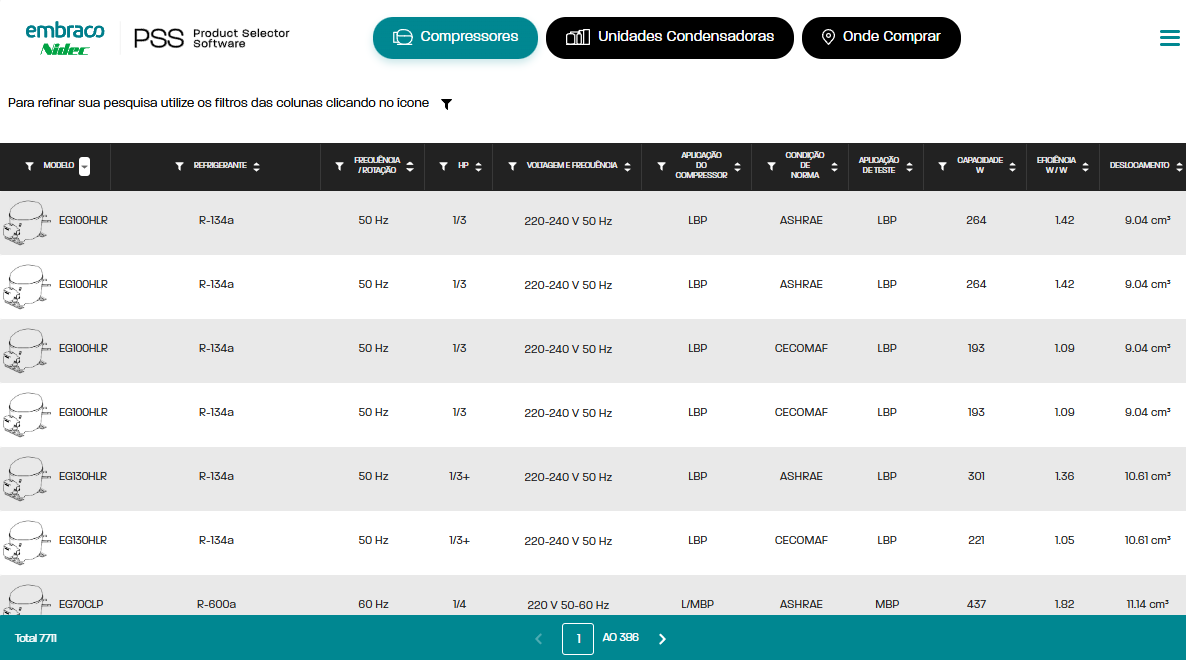
\includegraphics[width=0.8\linewidth]{Imagens/Desenvolvimento/PSS-embraco.png}
    \caption{Seletor de produtos}
    \label{fig:seletor de produtos}
\end{figure}


\newpage

\section{Ciclo de Refrigeração Padrão:}

    Com os dados preliminares obtidos, foi feita uma rotina em Python, para o cálculo 

\begin{equation}
    \dot{Q_L} = \dot{m}(h_1-h_4)
    \label{QL}
\end{equation}

\begin{equation}
    \dot{Q_H} = \dot{m}(h_2-h_3)
    \label{QH}
\end{equation}

\begin{equation}
    \dot{W_{comp}} = \dot{m}(h_2-h_1)
    \label{W compressor}
\end{equation}

\begin{equation}
    \Delta h_{1-2} \simeq  c_p (T_2-T_1)
    \label{simplificacao entalpia}
\end{equation}

\begin{equation}
    COP = \frac{T_H}{T_H - T_L}
    \label{COP carnot}
\end{equation}




